 
%% LyX 2.2.1 created this file.  For more info, see http://www.lyx.org/.
%% Do not edit unless you really know what you are doing.
\documentclass{article}\usepackage[]{graphicx}\usepackage[]{color}
% maxwidth is the original width if it is less than linewidth
% otherwise use linewidth (to make sure the graphics do not exceed the margin)
\makeatletter
\def\maxwidth{ %
  \ifdim\Gin@nat@width>\linewidth
    \linewidth
  \else
    \Gin@nat@width
  \fi
}
\makeatother

\definecolor{fgcolor}{rgb}{0.345, 0.345, 0.345}
\newcommand{\hlnum}[1]{\textcolor[rgb]{0.686,0.059,0.569}{#1}}%
\newcommand{\hlstr}[1]{\textcolor[rgb]{0.192,0.494,0.8}{#1}}%
\newcommand{\hlcom}[1]{\textcolor[rgb]{0.678,0.584,0.686}{\textit{#1}}}%
\newcommand{\hlopt}[1]{\textcolor[rgb]{0,0,0}{#1}}%
\newcommand{\hlstd}[1]{\textcolor[rgb]{0.345,0.345,0.345}{#1}}%
\newcommand{\hlkwa}[1]{\textcolor[rgb]{0.161,0.373,0.58}{\textbf{#1}}}%
\newcommand{\hlkwb}[1]{\textcolor[rgb]{0.69,0.353,0.396}{#1}}%
\newcommand{\hlkwc}[1]{\textcolor[rgb]{0.333,0.667,0.333}{#1}}%
\newcommand{\hlkwd}[1]{\textcolor[rgb]{0.737,0.353,0.396}{\textbf{#1}}}%
\let\hlipl\hlkwb

\usepackage{framed}
\makeatletter
\newenvironment{kframe}{%
 \def\at@end@of@kframe{}%
 \ifinner\ifhmode%
  \def\at@end@of@kframe{\end{minipage}}%
  \begin{minipage}{\columnwidth}%
 \fi\fi%
 \def\FrameCommand##1{\hskip\@totalleftmargin \hskip-\fboxsep
 \colorbox{shadecolor}{##1}\hskip-\fboxsep
     % There is no \\@totalrightmargin, so:
     \hskip-\linewidth \hskip-\@totalleftmargin \hskip\columnwidth}%
 \MakeFramed {\advance\hsize-\width
   \@totalleftmargin\z@ \linewidth\hsize
   \@setminipage}}%
 {\par\unskip\endMakeFramed%
 \at@end@of@kframe}
\makeatother

\definecolor{shadecolor}{rgb}{.97, .97, .97}
\definecolor{messagecolor}{rgb}{0, 0, 0}
\definecolor{warningcolor}{rgb}{1, 0, 1}
\definecolor{errorcolor}{rgb}{1, 0, 0}
\newenvironment{knitrout}{}{} % an empty environment to be redefined in TeX

\usepackage{alltt}
\usepackage[sc]{mathpazo}
\usepackage[T1]{fontenc}
\usepackage{geometry}
\geometry{verbose,tmargin=2.5cm,bmargin=2.5cm,lmargin=2.5cm,rmargin=2.5cm}
\setcounter{secnumdepth}{2}
\setcounter{tocdepth}{2}
\usepackage{url}
\usepackage{placeins}
\usepackage[unicode=true,pdfusetitle,
 bookmarks=true,bookmarksnumbered=true,bookmarksopen=true,bookmarksopenlevel=2,
 breaklinks=false,pdfborder={0 0 1},backref=false,colorlinks=false]
 {hyperref}
\hypersetup{
 pdfstartview={XYZ null null 1}}
\usepackage{breakurl}
\IfFileExists{upquote.sty}{\usepackage{upquote}}{}
\begin{document}


\title{Electricity usage and the COVID-19 pandemic}

\author{Nathaniel Bloomfield}

\maketitle

\section{Aims}

Comparing electricity usage patterns between years gives us an idea of how COVID-19 may have affected energy usage, but these changes in usage could also be due to other factors, such as differences in weather. Building a model based on previous years of electricity usage gives us a way to take these differences into account and compare the usage we'd expect given what we've observed previously and the usage that we are currently seeing during the COVID-19 pandemic. This will provide insights into how COVID-19 has affected the economy.

\section{Data}

To build a model we assembled a half hour electricity usage dataset that spanned from the start of 2015 to the 14th of October, 2020. Finding data with the required historical timeseries as well as being current to only the last couple of days was a challenge, but we were able to find temperature and solar radiation data and link these to the electricity usage data.Our electricity data was obtained from the Australian Energy Market Operator (AEMO) website, and provided \href{https://aemo.com.au/en/energy-systems/electricity/national-electricity-market-nem/data-nem/aggregated-data}{total electricity demand} for each state over half hour time periods. 

Given we have only state level aggregates for electricity usage, we found that we obtained better results with temperature data across each state, in addition to data from the capital cities. The \href{https://www.ncdc.noaa.gov/isd}{Integrated Surface Database} was able to supply hourly temperature data from weather stations to achieve this through the \texttt{worldmet} R package, but these stations had large numbers of missing values. We picked stations that had on average one record every six hours, and then linearly interpolated gaps of at-most six hours. Larger gaps of at-most a month were filled by taking a moving average individually for each hour of the day, and stations with larger data gaps were excluded. To match the electricity data, we linearly interpolated our hourly temperature data back to half-hourly values. The coverage of the stations overlayed with population density for NSW and VIC are shown in Figure \ref{fig:weatherstations}.

\begin{figure}[h]
\label{fig:weatherstations}
\centering
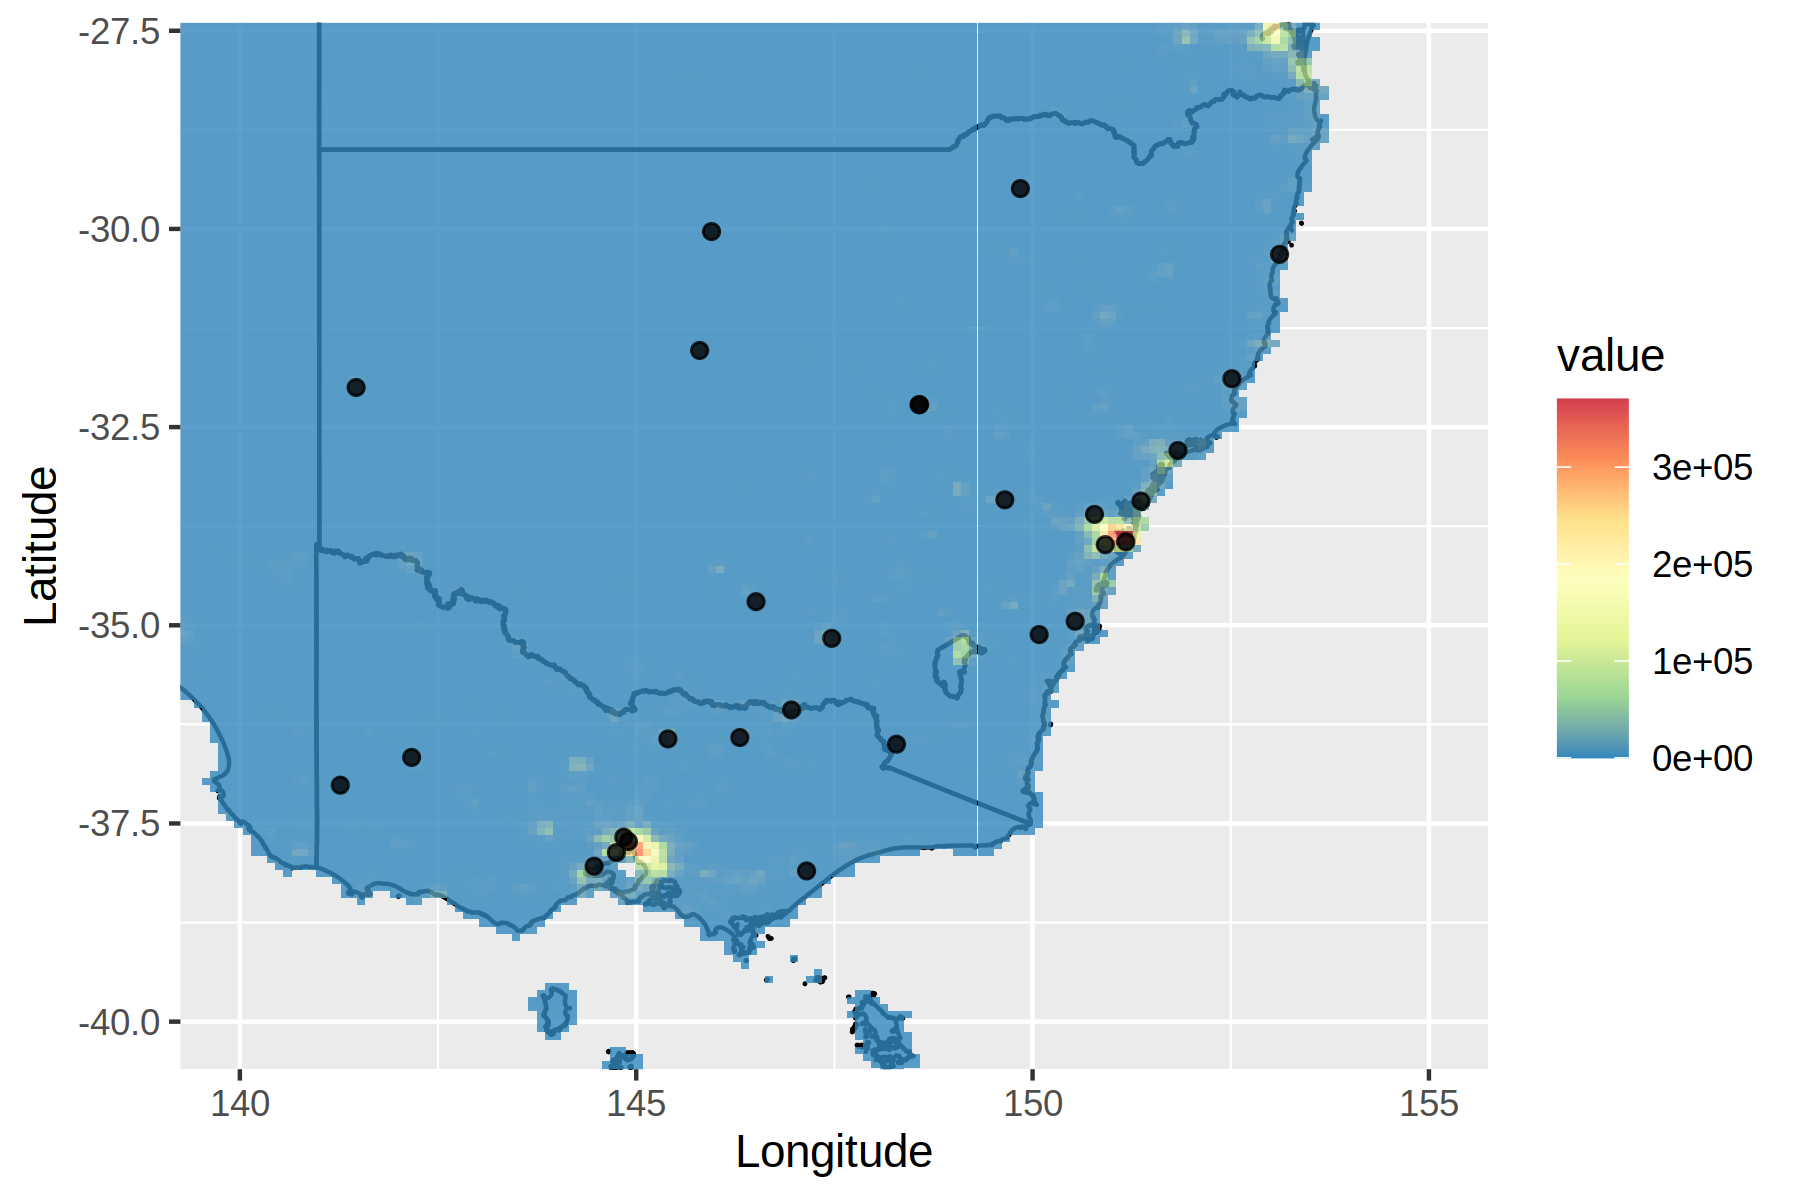
\includegraphics[width=1\textwidth]{figures/weather_station_map.png}
\caption{Black dots are the location of weather stations used for building models predicting electricity usage.}
\end{figure}

We also obtained gridded daily solar radiation data from \href{https://www.longpaddock.qld.gov.au/silo/gridded-data/}{SILO}, and extracted the values at each of the weather stations to provide reasonable coverage of each state. To approximate solar radiation at a half-hourly level, we used times for sunrise, noon and sunset from the \texttt{suncalc} R package based on the centroids of the weather station coordinates to first create an estimate of solar intensity throughout the day using a piece-wise sine curve based on these values. We then multiplied the daily solar radiation values at each weather station by this solar intensity appromixation to obtain a half-hourly approximation. This ignores the impact of cloud cover, but data with a higher temporal resolution was not available.

\FloatBarrier

\section{Model building}

\begin{figure}[h]
\label{fig:model_performance}
\centering
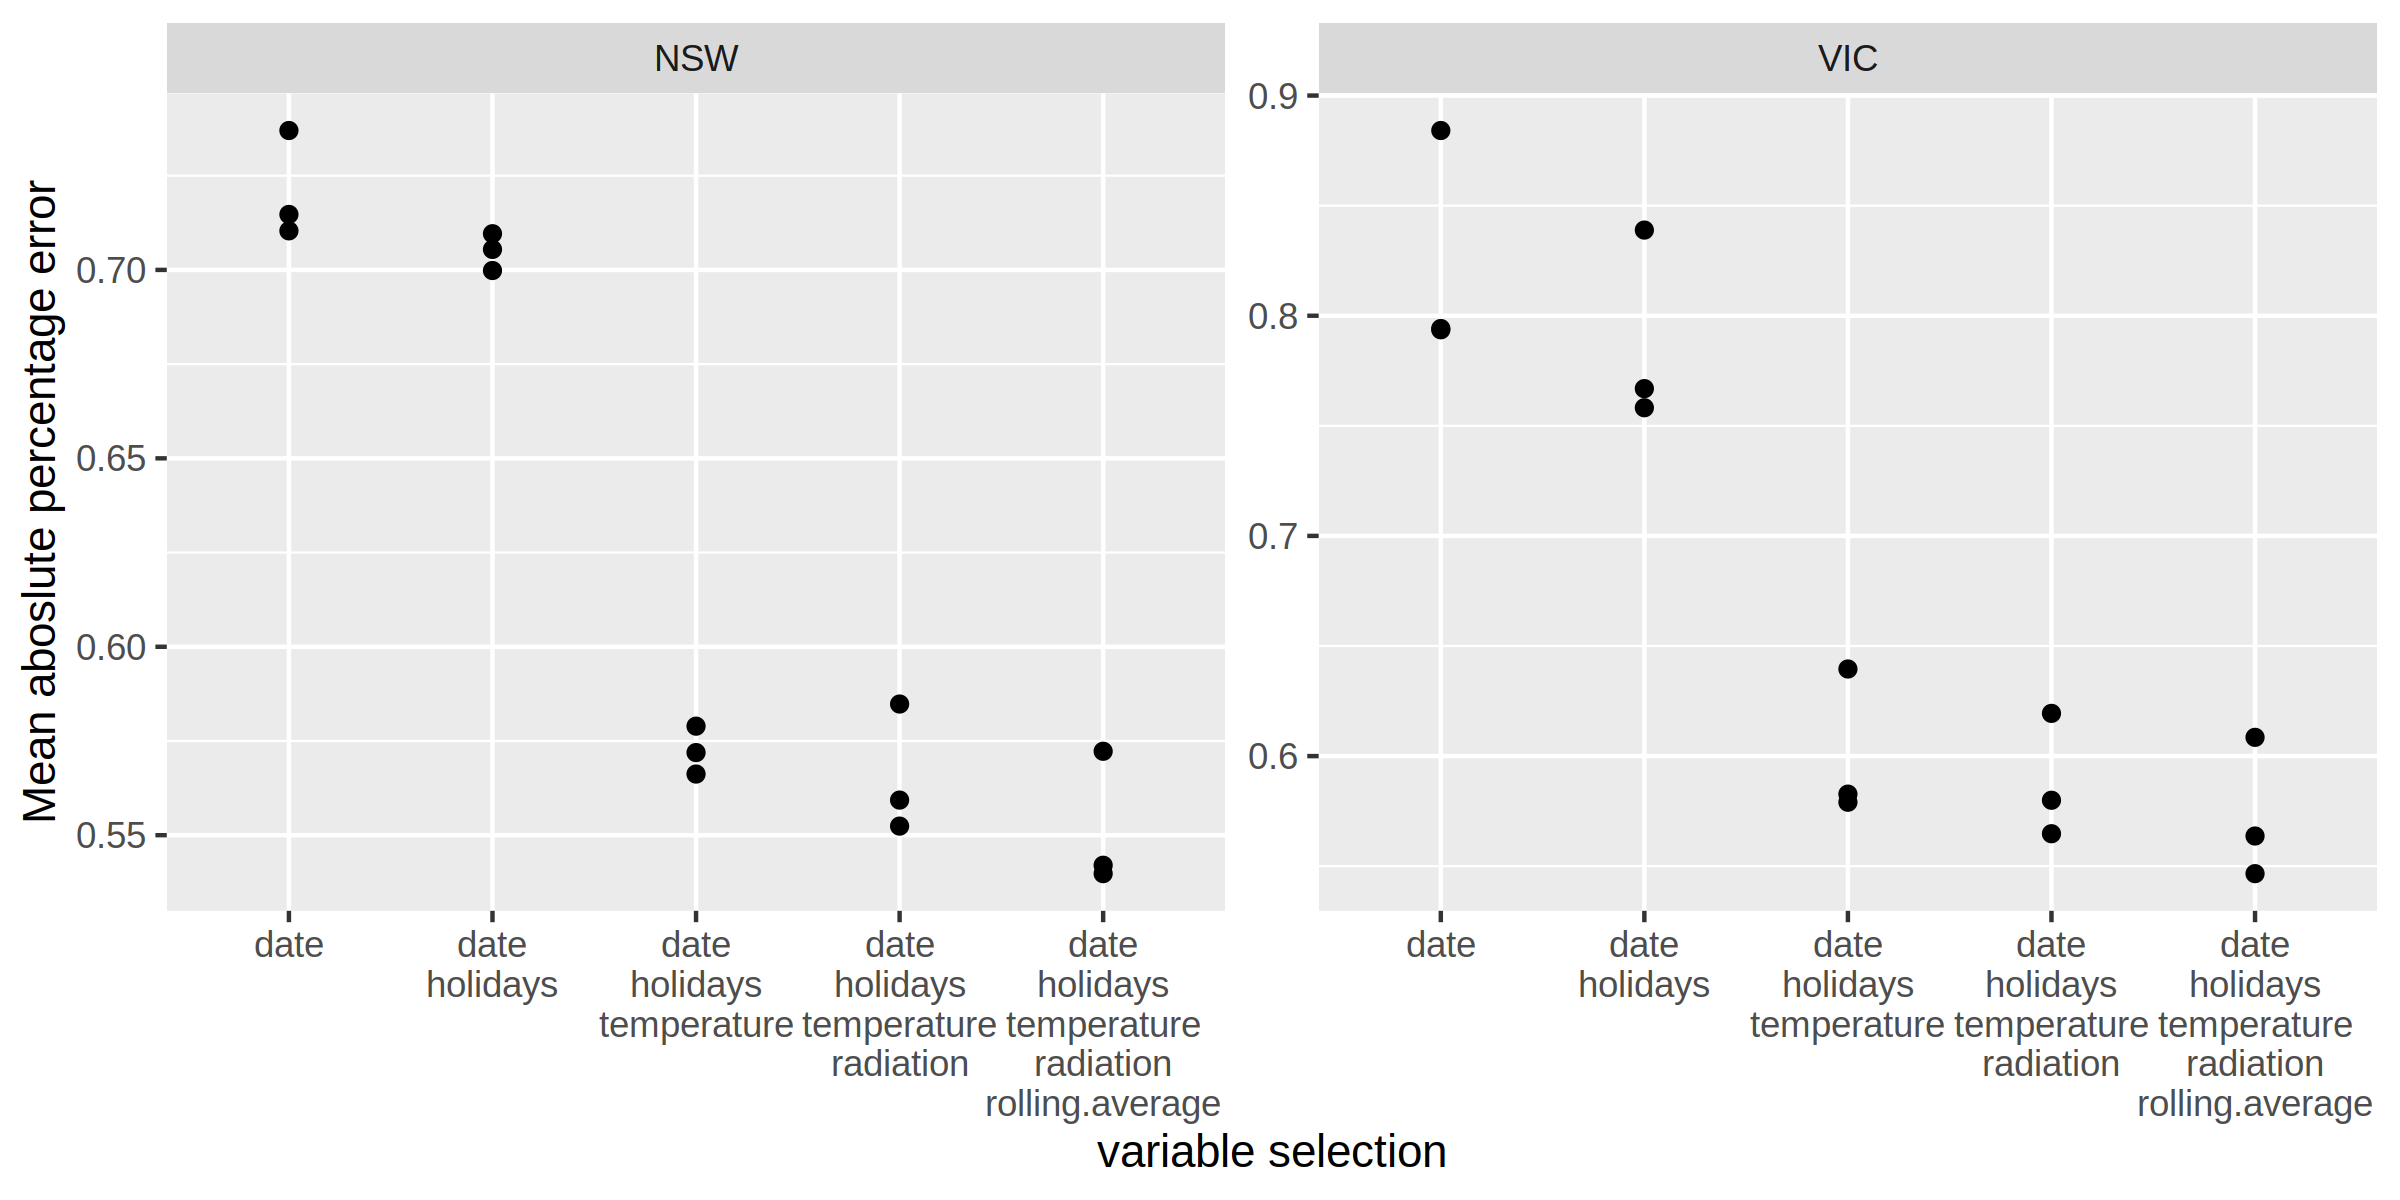
\includegraphics[width=1\textwidth]{figures/model_performance.png}
\caption{Model performance for VIC and NSW using different variable combinations. The three points are models tested on 2017, 2018 and 2019 data, but trained on all the preceding years.}
\end{figure}

\begin{figure}[h]
\label{fig:model_performance_raw}
\centering
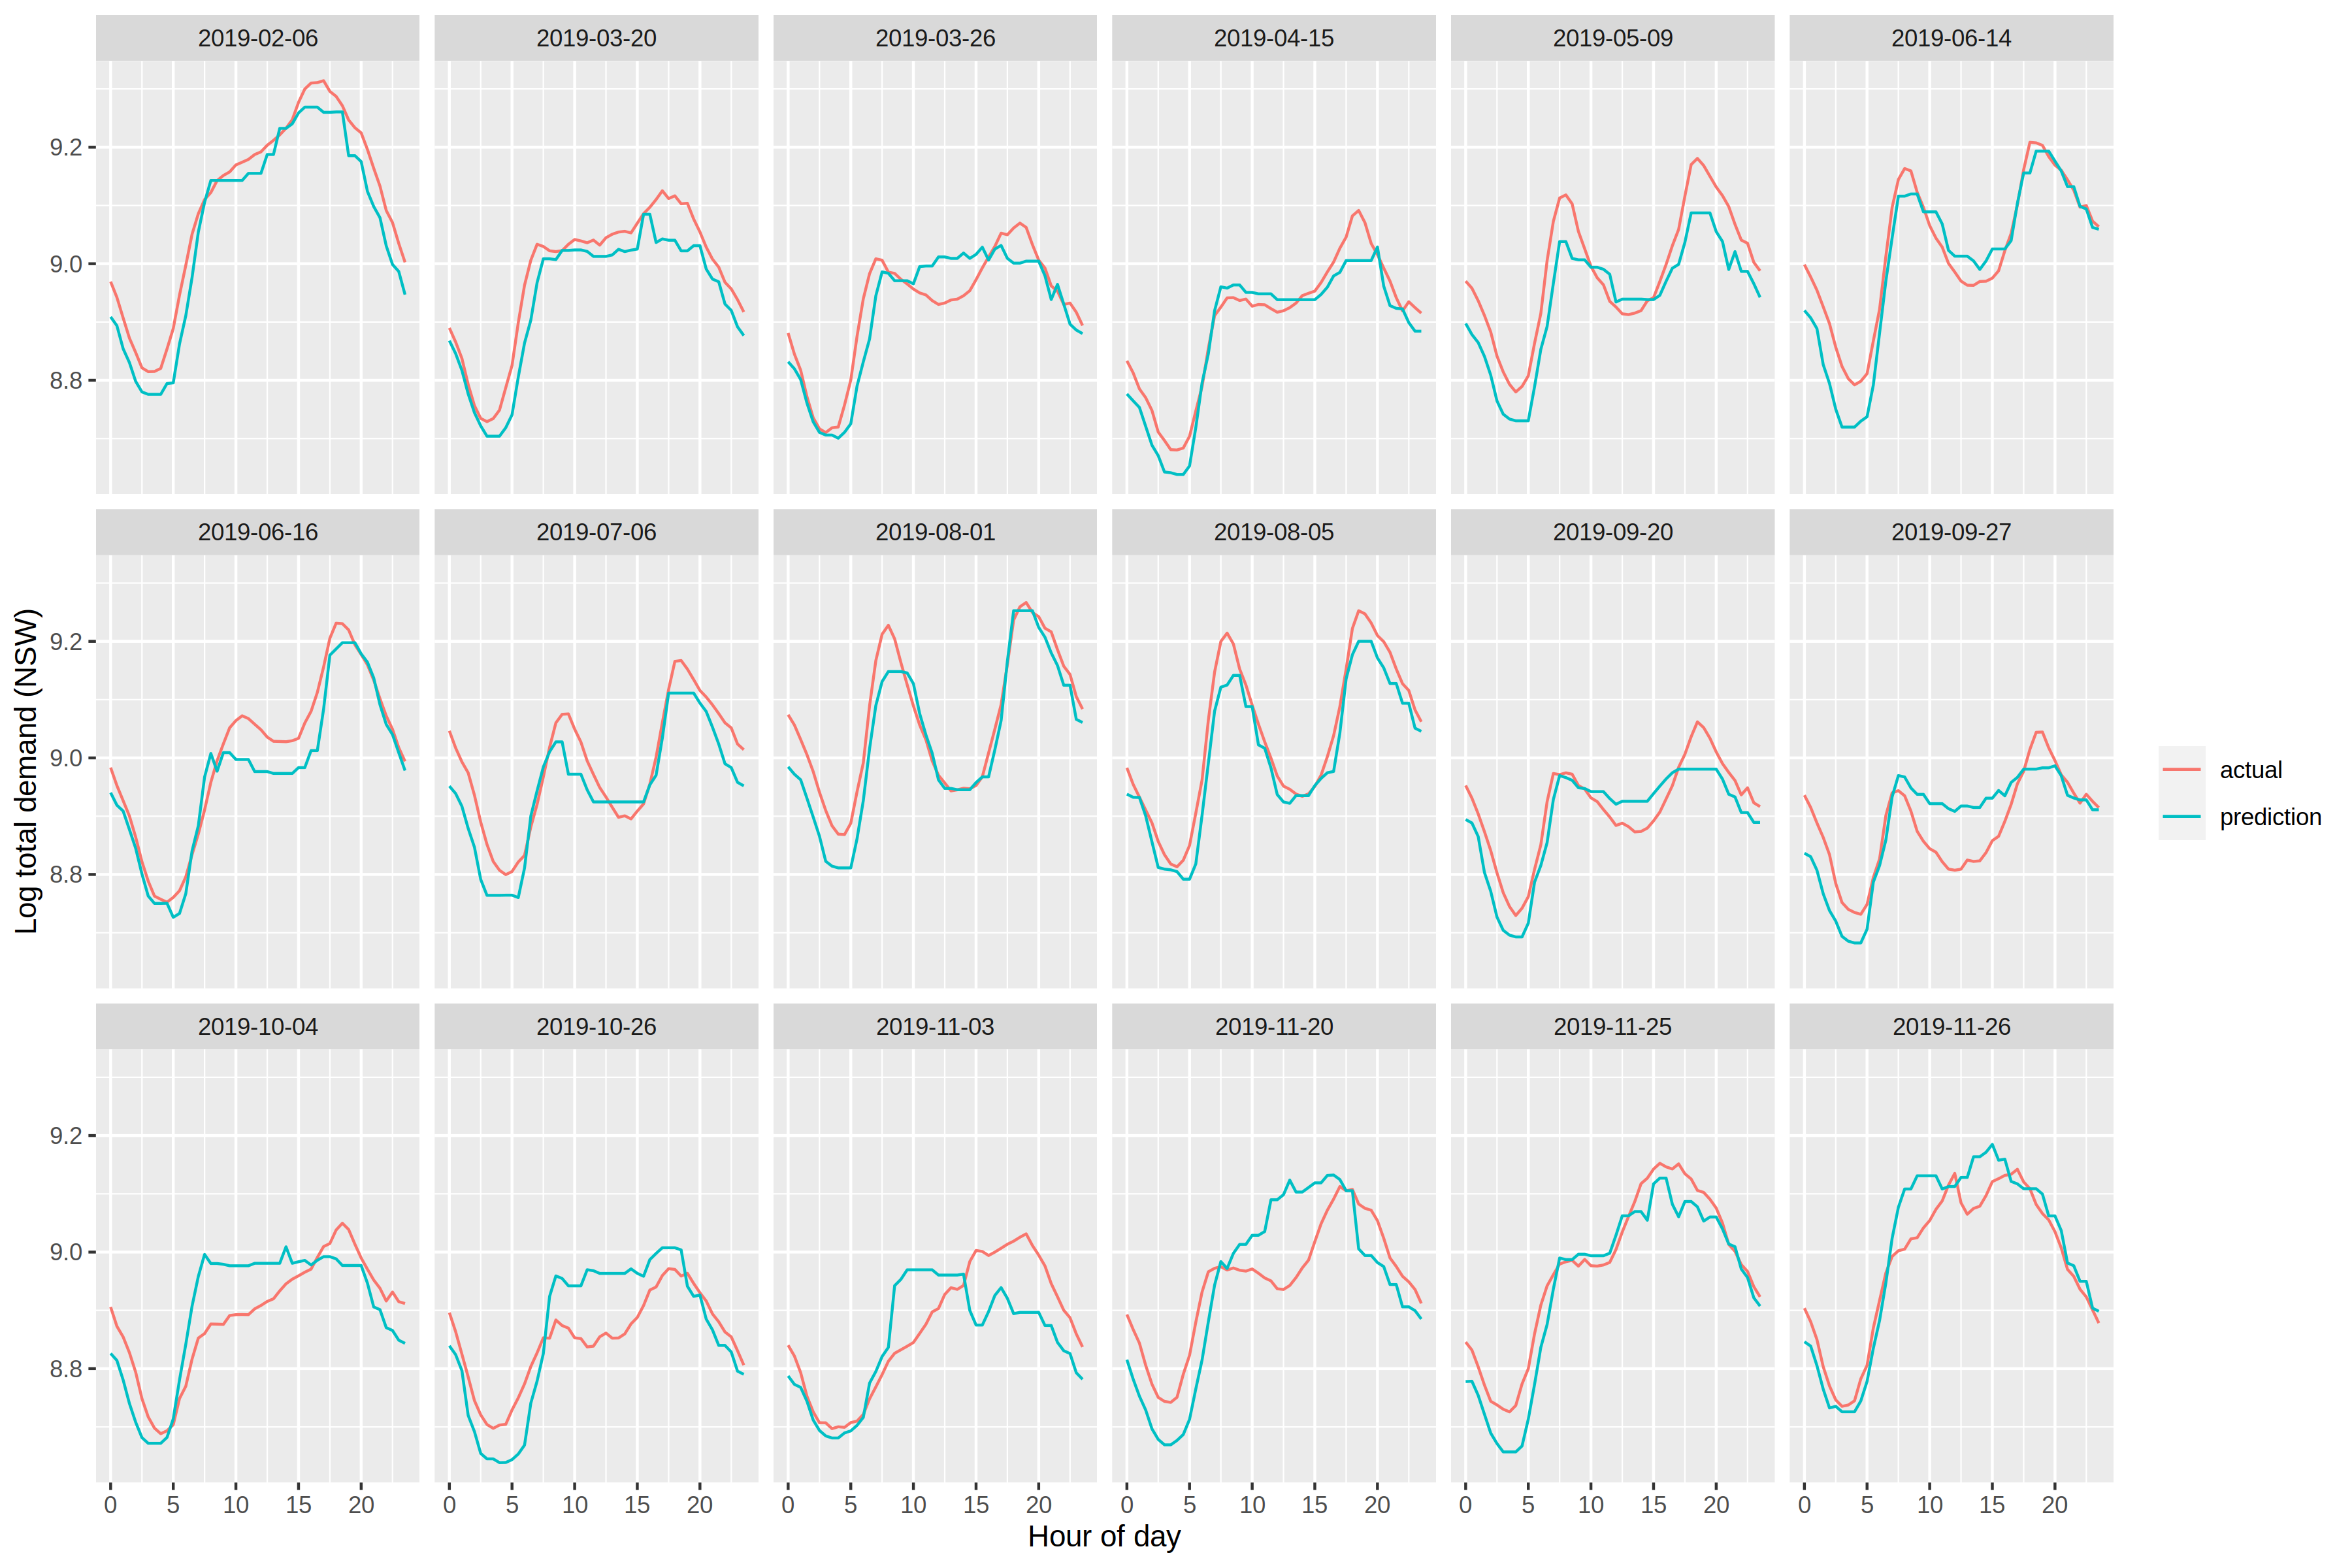
\includegraphics[width=1\textwidth]{figures/model_performance_raw.png}
\caption{Raw results of model trained on all predictors for NSW.}
\end{figure}

We used \texttt{xgboost} with the \texttt{tidymodels} framework in R to predict electricity usage. We grouped our predictor variables into five sets, and fit these in turn to see how they impacted the quality of the model. Date variables included the time of day, month, day of the week and a boolean variable describing if the day is a weekday. For holidays, we used the \texttt{holiday\_aus} function from the \texttt{tsibble} package, and again used a boolean value to describe them. We also included a variable that described the number of days to the closest holiday, previous or future. To describe temperature, we used the half-hourly temperature values from each weather station in the state as a variable. For solar radiation, we included both our approximate half-hourly solar radiation values at each weather station, as well as the piece-wise sine curve based on timing of sunrise and sunset. We also computed daily and weekly rolling averages of temperature and solar radiation.

The change in model performance as these variables are added is shown in Figure \ref{fig:model_performance} using mean absolute percentage error. Simply using dates to predict electricity usage provides a reasonable model and the error is reduced by 20-30\% when all the variables are included, with the largest impact being when temperature is included. Figure \ref{fig:model_performance_raw} shows some comparisons between actual usage and predicted usage for NSW in 2019, and shows that the log of total demand does not vary greatly over the day, staying between 8.7 and 9.3. For further results in this document, 2019 predictions are based on the model trained with data from 2015-2018, and 2020 predictions use a model trained on data from 2015-2019. 

\FloatBarrier
\section{Results}




\begin{figure}[h]
\label{fig:raw_demand}
\centering
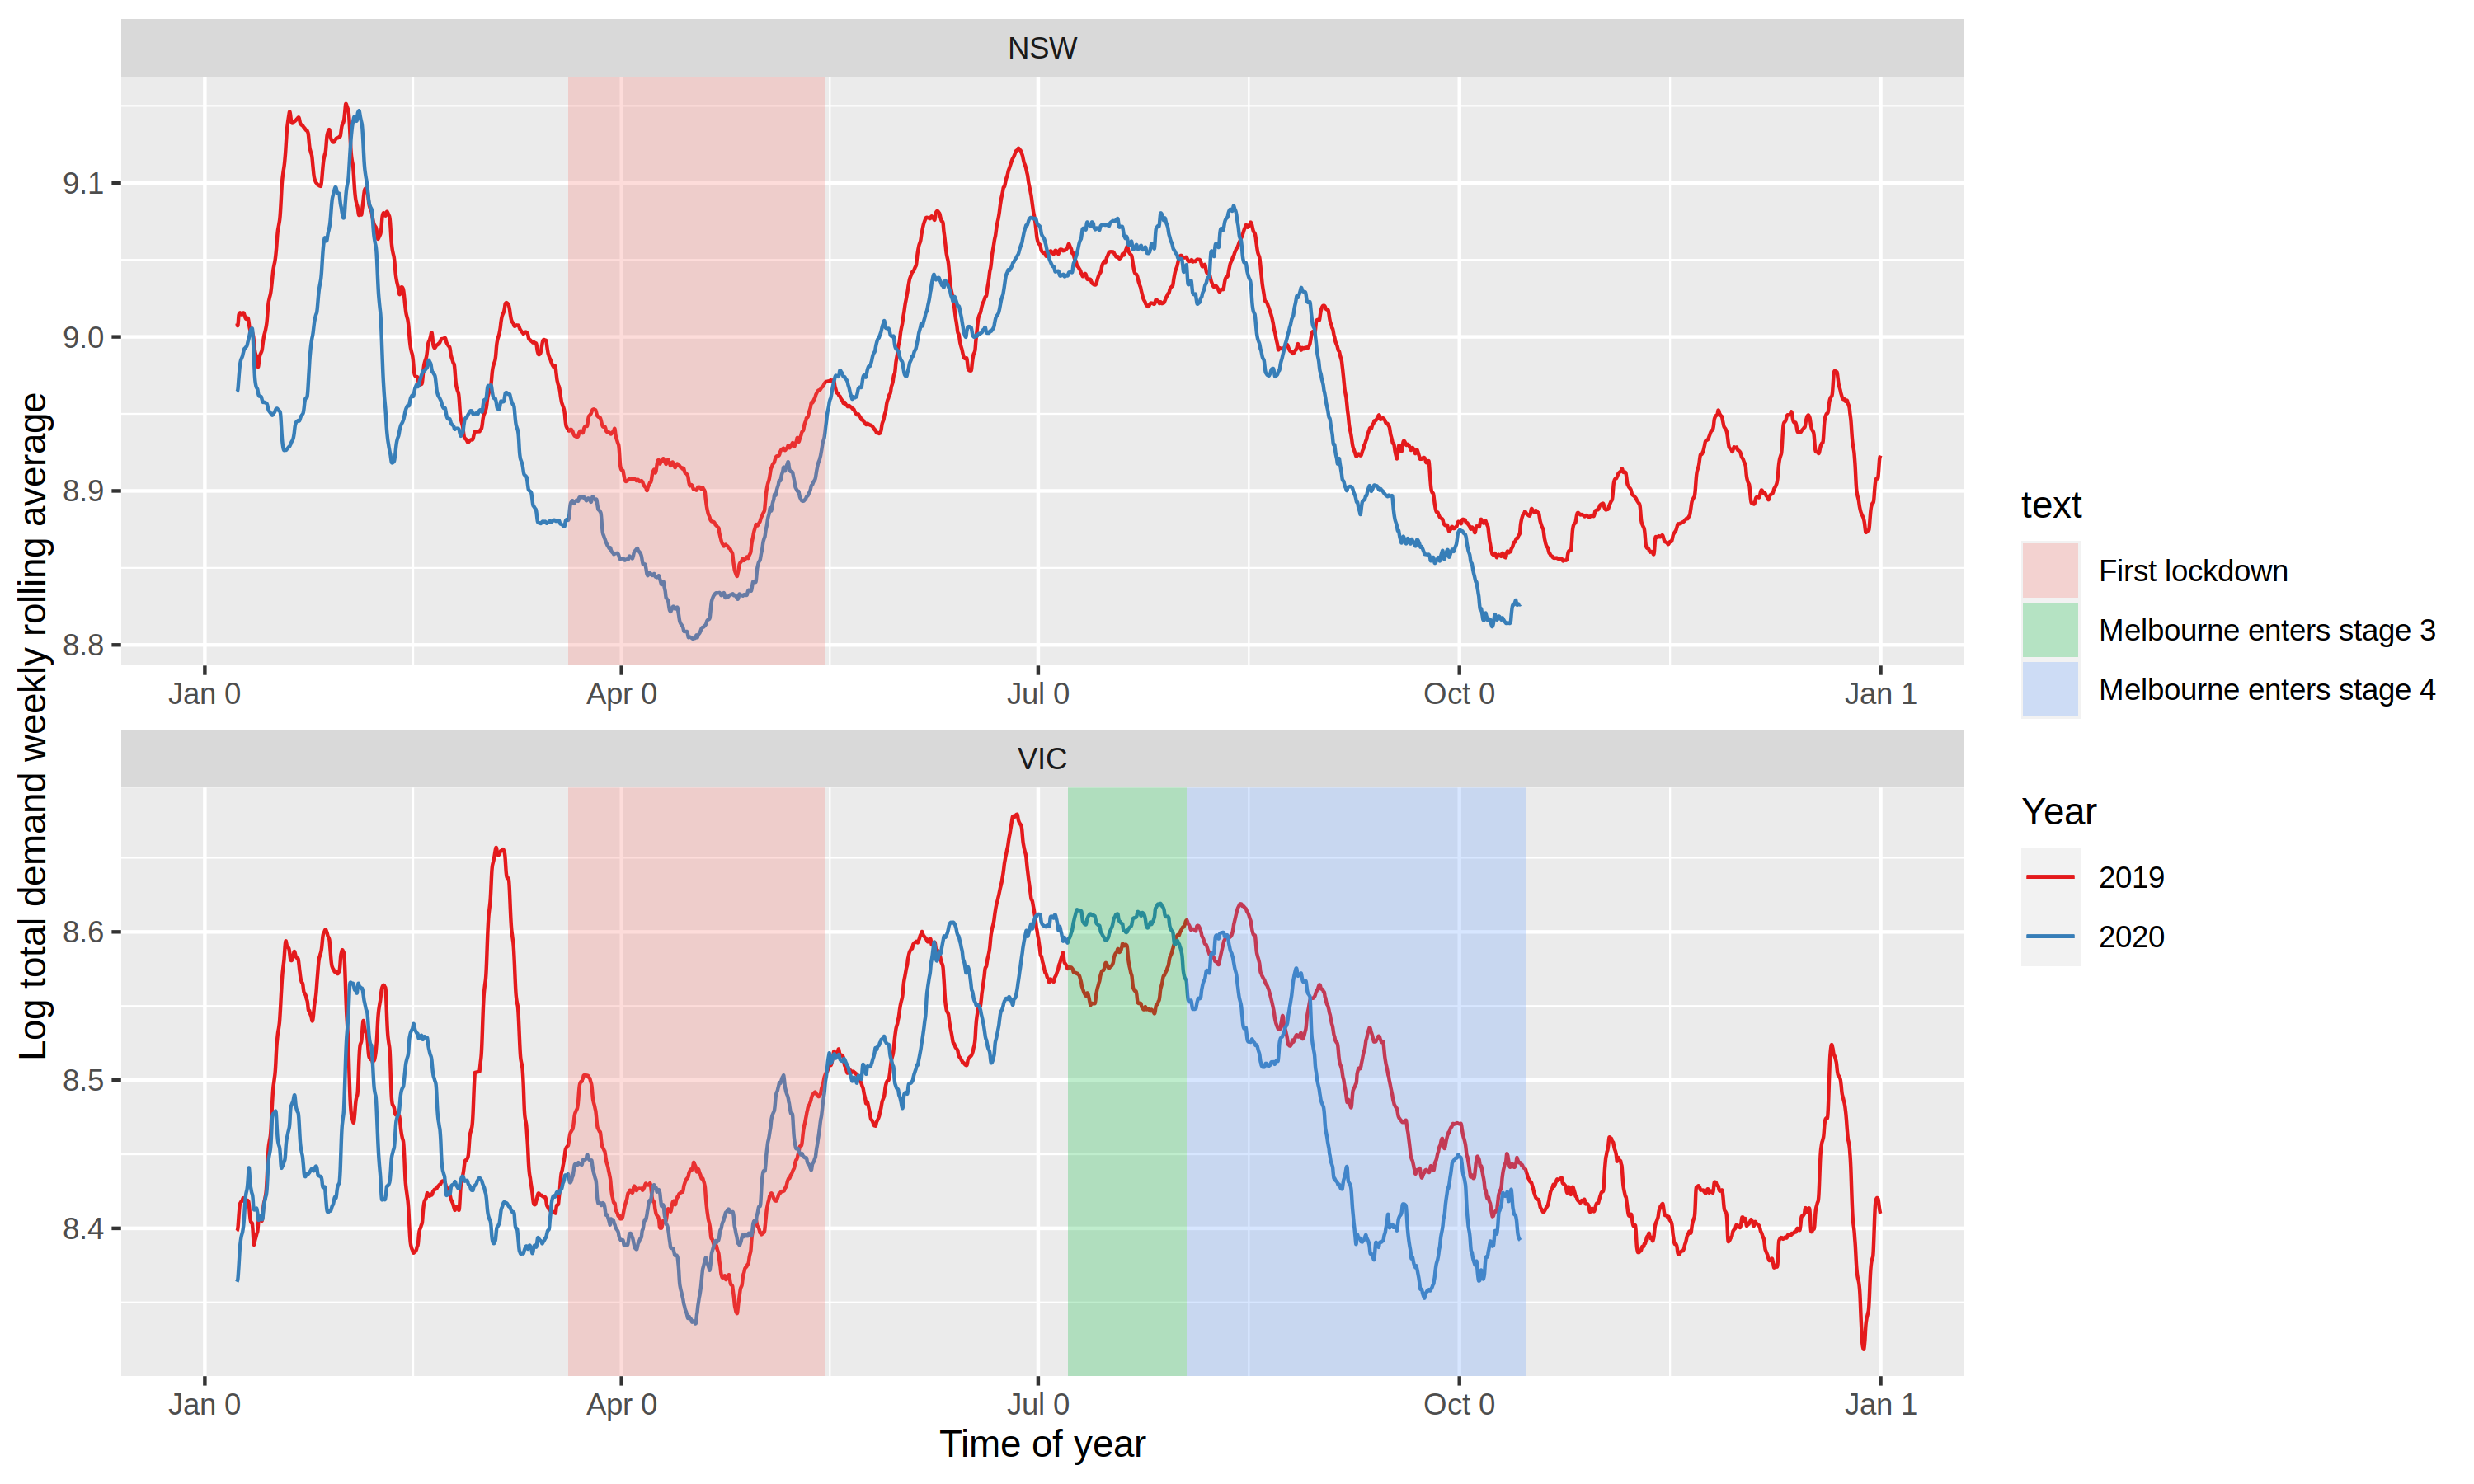
\includegraphics[width=1\textwidth]{figures/raw_demand.png}
\caption{Actual demand for 2019 and 2020 with the prediction for 2020 included as the dashed line, overlayed with approximate timing of major restrictions.}
\end{figure}

\begin{figure}[h]
\label{fig:demand_minus_pred}
\centering
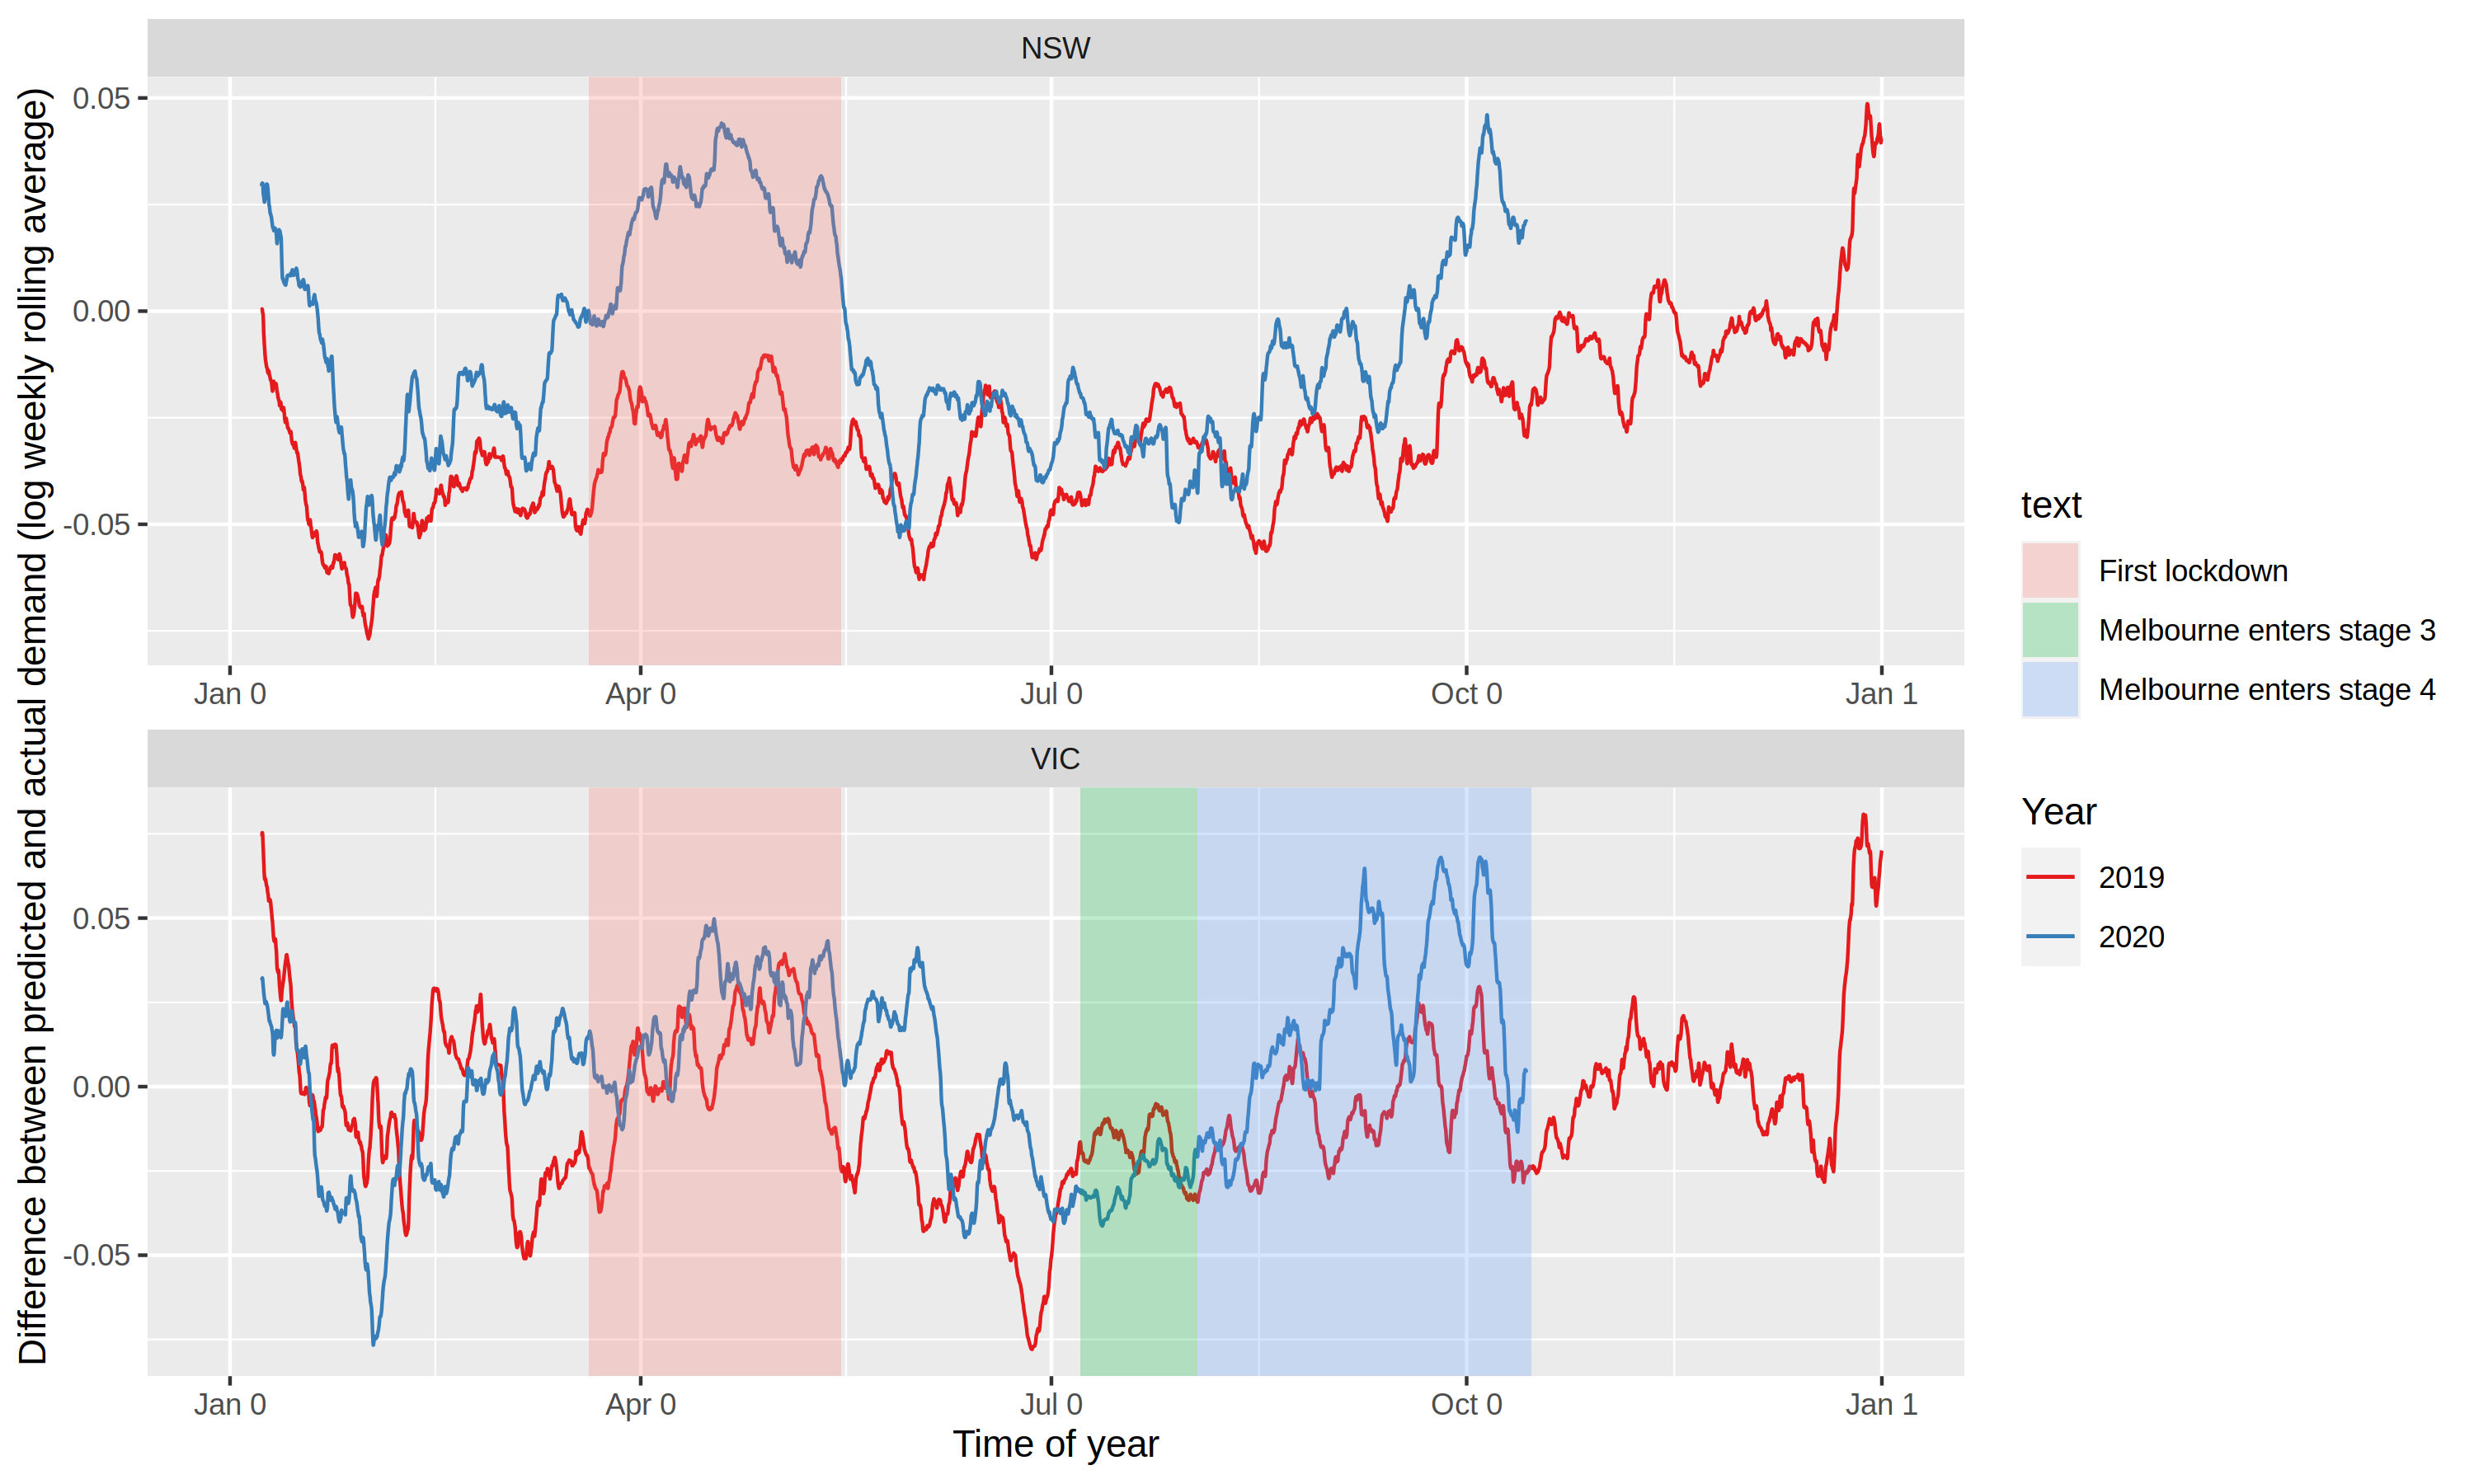
\includegraphics[width=1\textwidth]{figures/demand_minus_pred.png}
\caption{Difference between predictions and actual demand for 2019 and 2020, overlayed with approximate timing of major restrictions.}
\end{figure}


\begin{figure}[h]
\label{fig:unemployment}
\centering
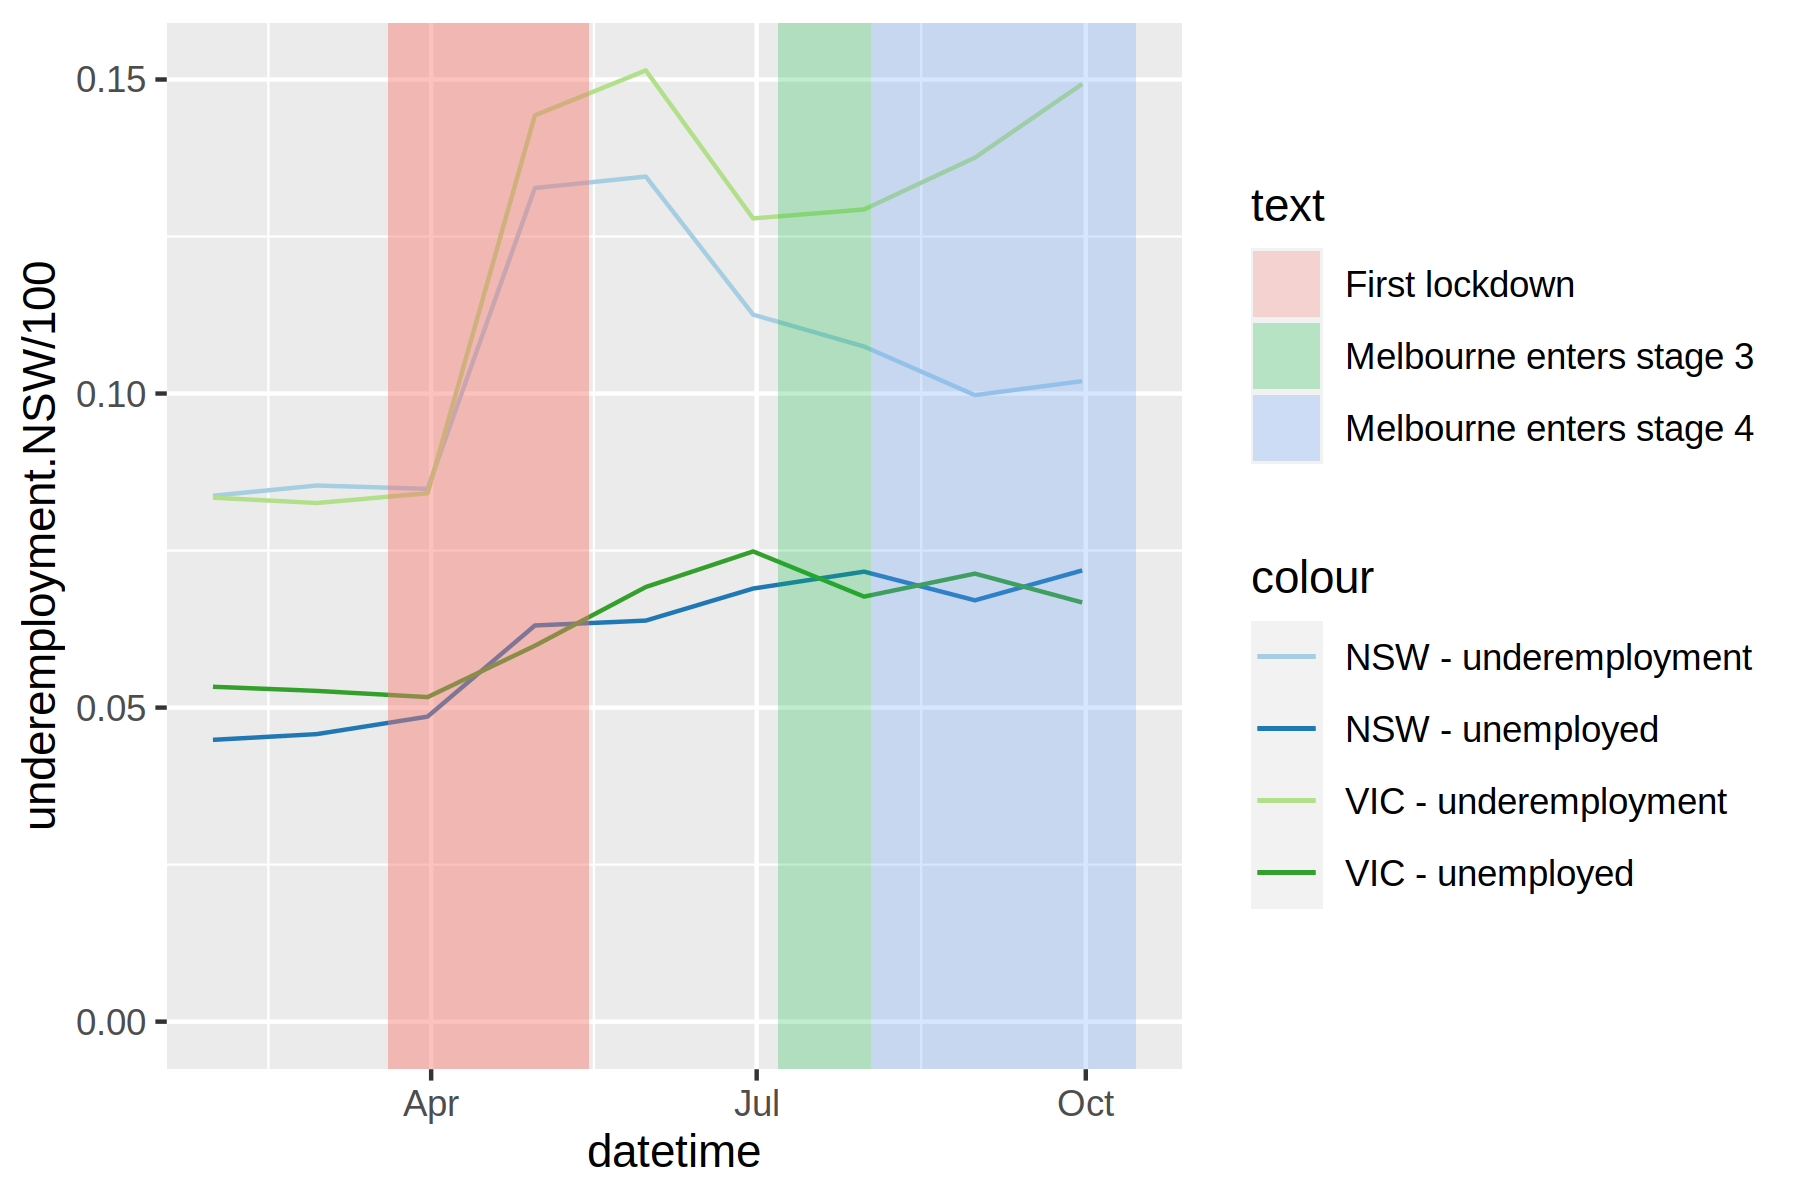
\includegraphics[width=1\textwidth]{figures/unemployment.png}
\caption{Unemployment data from the Australian Bureau of Statistics overlayed with the timing of major restrictions. Dashed lines are for NSW, and solid are for Victoria.}
\end{figure}


\end{document}
